\subsection{Trig Functions \& The Unit Circle}
\noindent
Imagine aa circle of radius 1 centered at the origin that we'll call the unit circle. The x and y coordinates of a point on the unit circle are completely determined by the angle $\theta$ in radians between the x-axis and a line from the origin to the point.\\

\noindent
The function $\cos{\theta}$ tells us x-coordinate of the point, while $\sin{\theta}$ tells us the y-coordinate of the point. The function $\tan{\theta} = \frac{\sin{\theta}}{\cos{\theta}}$ tells us the slope of the line from the origin to the point. Most of the trig functions have geometric interpretations as shown below. The most used ones are $\sin$, $\cos$, $\tan=\frac{\sin}{\cos}$, $\cot = \frac{\cos}{\sin}$, $\csc=\frac{1}{\sin}$, and $\sec=\frac{1}{\cos}$.

\begin{figure}[H]
	\label{unitCircle}
	\centering
	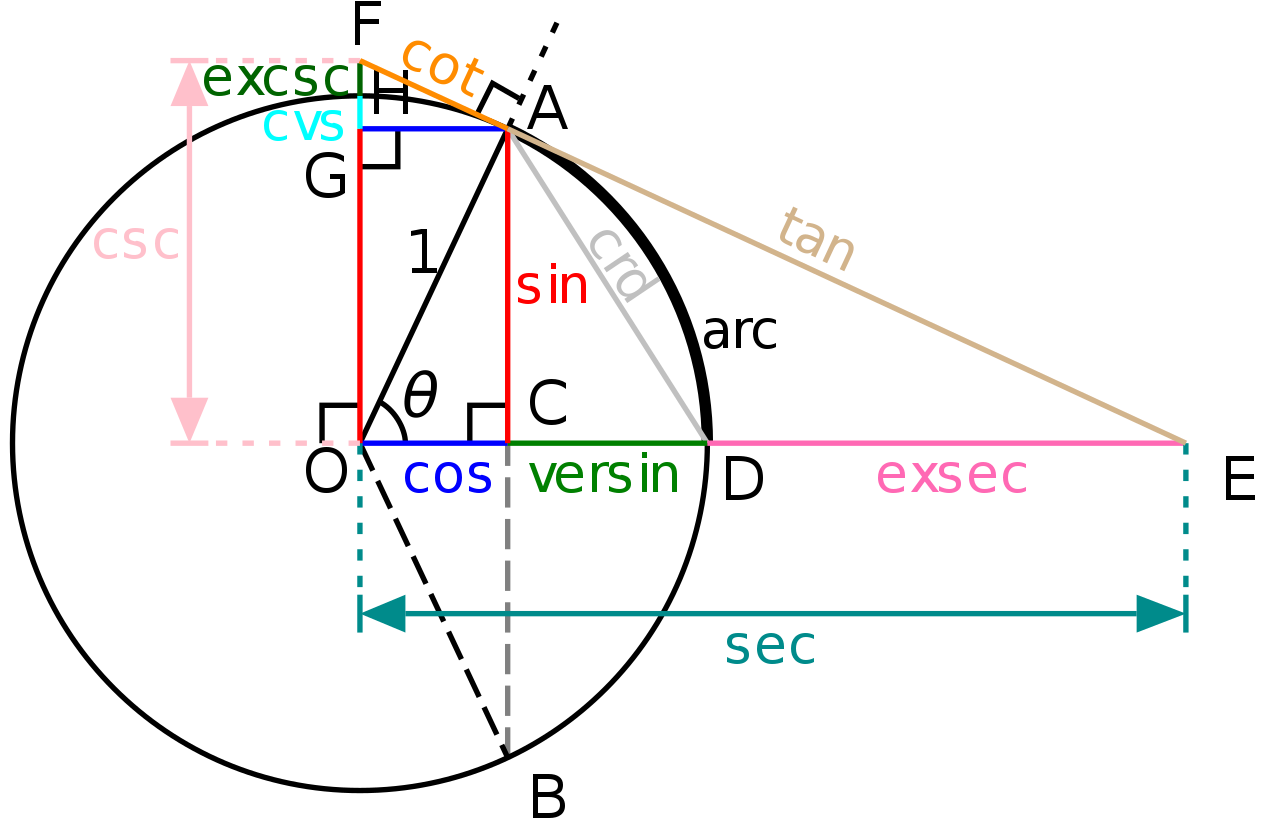
\includegraphics[width = 0.75\textwidth]{./backgroundReview/algebraPreCalc/unitCircle2.png}
	\caption{\hyperref{https://en.wikipedia.org/wiki/Unit_circle}{}{}{Wikipedia - Unit circle}}
\end{figure}

\noindent
We can also think about the inverses of these trig functions. These are either notated with a -1 exponent on the function, or the prefix arc in front of the function name. Many of these functions are only defined on a part of the domain $\left[0, 2\pi\right]$. Below is a table of the inverse trig functions and their domains.

\begin{table}[H]
	\centering
	\begin{tabular}{l|l}
		Function  & Domain                                                 \\ \hline
		$\arcsin$ & $\left[-1, 1\right]$           						   \\
		$\arccos$ & $\left[-1, 1\right]$                                   \\
		$\arctan$ & $\left(-\infty, \infty\right)$                         \\
		$\arccot$ & $\left(-\infty, \infty\right)$                         \\
		$\arccsc$ & $\left(-\infty, -1\right] \cup \left[1, \infty\right)$ \\
		$\arcsec$ & $\left(-\infty, -1\right] \cup \left[1, \infty\right)$
	\end{tabular}
\end{table}
